\documentclass[10pt,a4paper,twocolumn]{article}

\usepackage[margin=2cm,columnsep=0.75cm]{geometry}
\usepackage{booktabs}
\usepackage{graphicx}
\usepackage{caption}
\usepackage{amsmath}
\usepackage{balance}
\usepackage{fontspec}

\setmainfont{TeX Gyre Pagella}
\setsansfont{TeX Gyre Heros}

\captionsetup{font=small,labelfont=bf}
\usepackage{titlesec}
\titleformat{\section}{\sffamily\bfseries\large}{\thesection}{0.6em}{}
\titleformat{\subsection}{\sffamily\bfseries\normalsize}{\thesubsection}{0.6em}{}

\newcommand{\NumSamples}{188}
\newcommand{\NumCorrect}{180}
\newcommand{\AccTotal}{95.7\%}
\newcommand{\AccCILow}{91.8\%}
\newcommand{\AccCIHigh}{97.8\%}
\newcommand{\InputTokens}{122\thinspace404}
\newcommand{\OutputTokens}{8\thinspace460}
\newcommand{\TotalCost}{0.0051}
\newcommand{\NCertain}{134}
\newcommand{\PctCertain}{71.3\%}
\newcommand{\AccCertain}{99.3\%}
\newcommand{\NUncertain}{54}
\newcommand{\AccUncertain}{87.0\%}
\newcommand{\MeanProbCorrect}{0.99}
\newcommand{\MeanProbWrong}{0.83}
\newcommand{\NWrong}{8}
\newcommand{\LowBinN}{7}
\newcommand{\LowBinCorrect}{4}
\newcommand{\LowBinAcc}{57.1\%}
\newcommand{\ModelLetterA}{48}
\newcommand{\ModelLetterB}{41}
\newcommand{\ModelLetterC}{53}
\newcommand{\ModelLetterD}{46}
\newcommand{\KeyLetterA}{47}
\newcommand{\KeyLetterB}{42}
\newcommand{\KeyLetterC}{51}
\newcommand{\KeyLetterD}{48}


\title{\sffamily JEV-1.13 on High School U.S. History: Test Report}
\author{}
\date{September 28, 2026}

\begin{document}
\maketitle

\section*{Abstract}
This report presents the results of the model JEV-1.13 on the high school
U.S. history subject of the MMLU benchmark. The test comprises \NumSamples{}
four-option multiple-choice questions; the model answered \NumCorrect{}
correctly, an accuracy of \AccTotal{}, far above the 25\% random-guessing
level. The model also states a probability for every option: the probability
assigned to the chosen option (the chosen probability) was 1.00 for
\NCertain{} questions, which were almost all correct (\AccCertain{}), and
below 1.00 for \NUncertain{} questions, which were \AccUncertain{} correct.
The whole test consumed \InputTokens{} input tokens and
\OutputTokens{} output tokens, costing USD \TotalCost{} in total. In this
scenario the model answers accurately at very low cost, and its chosen
probability indicates how reliable an answer is.

\section{Dataset}
The data come from the test split of the high school U.S. history subject of
the MMLU (Massive Multitask Language Understanding) benchmark~\cite{mmlu}. The test
consists of \NumSamples{} four-option single-answer questions. Each item
presents a passage of material (a quoted document or a situational
description) followed by a question; the model must select the one correct
option. The answer keys provided by the dataset are distributed nearly
uniformly across
the four letters (A \KeyLetterA{}, B \KeyLetterB{}, C \KeyLetterC{}, D
\KeyLetterD{}). The subject under test is the model JEV-1.13 (identifier
\texttt{typesafe/jev-1.13-20260917}).

\section{Results}
All questions are scored against the answer key provided by the dataset.

\subsection{Overall Results}
Table~\ref{tab:overall} summarizes the overall outcome. Of the \NumSamples{}
questions, the model answered \NumCorrect{} correctly, an accuracy of
\AccTotal{} (95\% confidence interval \AccCILow{}--\AccCIHigh{}). Random
guessing on four-option questions yields 25\% on average, so the model scores
far above chance.

\begin{table}[htbp]
  \centering
  \caption{Overall results}
  \label{tab:overall}
  \begin{tabular}{lc}
    \toprule
    Item & Value \\
    \midrule
    Questions & \NumSamples \\
    Correct & \NumCorrect \\
    Accuracy & \AccTotal \\
    95\% confidence interval & \AccCILow{}--\AccCIHigh \\
    \bottomrule
  \end{tabular}
\end{table}

\subsection{Chosen Probability and Accuracy}
Besides the selected option, the model states a probability for each of the
four options; the probability assigned to that option is called the chosen
probability.

For \NCertain{} questions (\PctCertain{}) the chosen probability was 1.00,
and \AccCertain{} of them were answered correctly; for the remaining
\NUncertain{} questions it was below 1.00, with \AccUncertain{} accuracy.
The chosen probability averages \MeanProbCorrect{} on the \NumCorrect{}
correct answers and \MeanProbWrong{} on the \NWrong{} wrong ones.

Figure~\ref{fig:prob} groups questions by chosen probability. Only
\LowBinCorrect{} of the \LowBinN{} questions below 0.90 were correct;
accuracy rises across the bands overall and exceeds 99\% in the 0.99 and
1.00 bands. The chosen probability therefore separates reliable answers from
unreliable ones and can serve as a reference for deciding whether to trust an
individual answer.

\begin{figure}[htbp]
  \centering
  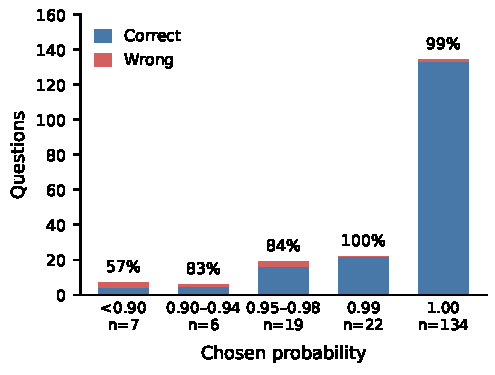
\includegraphics[width=\columnwidth]{figures/fig_prob_en.pdf}
  \caption{Question counts and accuracy by chosen-probability band. Bar height
  is the number of questions in the band (blue: correct, red: wrong); the
  percentage above each bar is the accuracy of that band.}
  \label{fig:prob}
\end{figure}

\subsection{Cost}
As Table~\ref{tab:cost} shows, the whole test consumed \InputTokens{} input
tokens and \OutputTokens{} output tokens, costing USD \TotalCost{} in total.

\begin{table}[htbp]
  \centering
  \caption{Cost of the test}
  \label{tab:cost}
  \begin{tabular}{lc}
    \toprule
    Item & Amount \\
    \midrule
    Input tokens & \InputTokens \\
    Output tokens & \OutputTokens \\
    Total cost & USD \TotalCost \\
    \bottomrule
  \end{tabular}
\end{table}

\balance
\section{Conclusion}
On \NumSamples{} high school U.S. history multiple-choice questions, JEV-1.13
answered \NumCorrect{} correctly, an accuracy of \AccTotal{}, far above the
random level. More than seventy percent of its answers had a chosen
probability of 1.00 and were almost all correct, while answers below 0.90
were correct less than sixty percent of the time. The entire test cost about
half a U.S. cent. Overall, in this scenario JEV-1.13 answers accurately at
very low cost, and its chosen probability can be used to flag unreliable
answers.

\begin{thebibliography}{9}
\bibitem{mmlu}
Dan Hendrycks, Collin Burns, Steven Basart, Andrew Critch, Jerry Li, Dawn
Song, Jacob Steinhardt.
\emph{Measuring Massive Multitask Understanding}.
ICLR 2021. Data taken from the \texttt{cais/mmlu} test split.
\end{thebibliography}

\end{document}
